\documentclass{article}
\usepackage{../../math_template}

\author{Jonathan Kasongo}
\title{Noether Sheet 8}

\begin{document}
\maketitle
\centerline{
These were my solutions to the Noether Mentoring Scheme Sheet 8. Problem
statements are abridged.
}

\begin{problem}{Problem 1}
Suppose that
$$
x^2 - 3ax + b = 0 \text{ has solutions } x=c \text{ and } x=d, \text{ and }
$$
$$
x^2 + cx + d = 0 \text{ has solution } x=a \text{ and } x=b.
$$
All of $a,b,c$ and $d$ are non-zero. What are the possible values of
$a,b,c$ and $d$?
\end{problem}

\begin{solution}{Solution}
Vieta's formulae give us the following relations
\[
\begin{aligned}
3a &= c + d, \quad &b = cd \\
-c &= a + b, \quad &d = ab
\end{aligned}
\]
Using the two equations on the right we find that
$$
b = c(ab) \iff ac = 1 \ (\text{Since } b\neq0)
$$
Now observe
\[
\begin{aligned}
3a &= c + d\\
&= c + (ab)\\
&= c + a(-a-c)\\
&= c - ac - a^2\\
&= c - (1) - a^2 \\
3a^2 &= (ac) - a - a^3\\
&= 1 - a - a^3
\end{aligned}
\]
So $a$ satisfies $a^3 + 3a^2 + a - 1 = 0$. By inspection $a = -1$ is a
root. Now we can use polynomial long division to find that
$$
(a+1)(a^2 + 2a - 1) = 0
$$
so $a \in \{-1, \ -1+\sqrt2, \ -1-\sqrt2 \}$.
\\

% should really only need to show that vietas relations hold
\textit{Case 1: $a=-1$.} Then $c = -1$. Also $d = 3(-1) - (-1) = -2$.
Finally $b = -(-1) - (-1) = 2$. Let's check that this works,
$$
3(-1) = (-1) + (-2), \quad 2 = (-1)(-2)
$$
$$
-(-1) = (-1) + (2), \quad -2 = (-1)(2)
$$
so $(a,b,c,d)=(-1,2,-1,-2)$ is a solution. \\

\textit{Case 2: $a = -1 + \sqrt2$.} Then $c = 1/(-1 + \sqrt2) = 1+\sqrt2$.
Also $d = 3(-1 + \sqrt2) - (1 + \sqrt2) = -4 + 2\sqrt2$. Finally
$b = -(-1 + \sqrt2) - (1 + \sqrt2) = - 2\sqrt2$. Let's check that it
works.
$$
3(-1 + \sqrt2) = (1 + \sqrt2) + (-4 + 2\sqrt2), \quad
-2\sqrt2 = (1+\sqrt2)(-4+2\sqrt2)
$$
$$
-(1 + \sqrt2) = (-1+\sqrt2) + (-2\sqrt2), \quad
-4 + 2\sqrt2 = (-1+\sqrt2)(-2\sqrt2)
$$
so $(a,b,c,d) = (-1+\sqrt2, \ -2\sqrt2, \ 1+\sqrt2, \ -4+2\sqrt2)$
is a solution.
\\

\textit{Case 3: $a = -1 - \sqrt2$.} Then $c = 1/(-1-\sqrt2) = 1-\sqrt2$.
Also $d = 3(-1-\sqrt2) - (1-\sqrt2) = -4 - 2\sqrt2$. Finally
$b = -(-1-\sqrt2) - (1-\sqrt2) = 2\sqrt2$. Let's check that
$$
3(-1-\sqrt2) = (1-\sqrt2) + (-4 - 2\sqrt2), \quad
2\sqrt2 = (1-\sqrt2)(-4-2\sqrt2)
$$
$$
-(1-\sqrt2) = (-1-\sqrt2) + (2\sqrt2), \quad
-4-2\sqrt2 = (-1-\sqrt2)(2\sqrt2)
$$
so $(a,b,c,d) = (-1-\sqrt2, \ 2\sqrt2, \ 1-\sqrt2, \ -4-2\sqrt2)$
is a solution. $\blacksquare$
\end{solution}
\newpage

\begin{problem}{Problem 2}
A square field has vertices at $(0,0), (9a, 0), (0, 9a)$ and $(9a, 9a)$.
A point $P$ is selected in the field, and three walls are drawn to the
edge of the field, dividing it into two triangles and a quadrilateral.
All three regions have the same area.\vspace{0.2cm}

How many possible locations of $P$ are there?
\end{problem}

\begin{solution}{Solution}
(Sketch of solution.) The answer is that there are four locations for $P$.
The three walls must each be to vertices of the square
because otherwise we won't have a quadrilateral but some other $n$-gon
($n > 4$). Consider the diagram where $A = (0,0)$ is the bottom left
corner of the square.

\begin{center}
\begin{asy}
/* Geogebra to Asymptote conversion, documentation at artofproblemsolving.com/Wiki go to User:Azjps/geogebra */
import graph; size(180);
real labelscalefactor = 0.5; /* changes label-to-point distance */
pen dps = linewidth(0.7) + fontsize(10); defaultpen(dps); /* default pen style */
pen dotstyle = black; /* point style */
real xmin = -0.389760132454166, xmax = 11.25470699736959, ymin = -0.8734186090228555, ymax = 11.6620042784344;  /* image dimensions */

pair A = (0.,0.), B = (9.,0.), C = (9.,9.), D = (0.,9.), P = (6.,6.), R = (6.,9.), Q = (9.,6.);
pair m_PQp = (3,6), m_PQ = (7.5, 6), m_PRp = (6, 3), m_PR = (6, 7.5);
/* draw figures */
draw(D--C);
draw(C--B);
draw(B--A);
draw(A--D);
draw(P--B);
draw(P--C);
draw(P--D);
draw(R--P,  linetype("4 4"));
draw(P--Q,  linetype("4 4"));
draw((0.,6.)--P,  linetype("4 4"));
draw(P--(6.,0.),  linetype("4 4"));
/* dots and labels */
dot(A,dotstyle);
label("$A$", (0.059292252264823916,0.1447554313715542), NE * labelscalefactor);
dot(B,dotstyle);
label("$B$", (9.05761710906097,0.1447554313715542), NE * labelscalefactor);
dot(C,dotstyle);
label("$C$", (9.05761710906097,9.15825452907291), NE * labelscalefactor);
dot(D,dotstyle);
label("$D$", (0.059292252264823916,9.15825452907291), NE * labelscalefactor);
dot(P,dotstyle);
label("$P$", (6.0531174098271805,6.153754829839125), NE * labelscalefactor);
dot(R,dotstyle);
label("$R$", (6.0531174098271805,9.15825452907291), NE * labelscalefactor);
dot(Q,dotstyle);
label("$Q$", (9.05761710906097,6.153754829839125), NE * labelscalefactor);
dot((6.,0.),dotstyle);
label("$R'$", (6.0531174098271805,0.1447554313715542), NE * labelscalefactor);
dot((0.,6.),dotstyle);
label("$Q'$", (0.059292252264823916,6.153754829839125), NE * labelscalefactor);

label("$9a-x$", m_PQp, S * labelscalefactor);
label("$9a-x$", m_PRp, W * labelscalefactor);
label("$x$", m_PR, NW * labelscalefactor);
label("$x$", m_PQ, S * labelscalefactor);

clip((xmin,ymin)--(xmin,ymax)--(xmax,ymax)--(xmax,ymin)--cycle);
/* end of picture */
\end{asy}
\end{center}

Note that $PQ = RP$ because the two triangles $\triangle DCP$ and
$\triangle BPC$ have the same base length and the same area, so their
perpendicular heights must also be the same. We call this length $x$.
\vspace{0.2cm}

The area of each triangle is $\frac12 9ax$. The area of the
quadrilateral is $\frac12 9a(9a-x) + \frac12 9a(9a-x)$. Since all three regions have equal areas,
\[
\begin{aligned}
\frac12 9ax &= 9a(9a-x) \\
x &= 2(9a-x) \\
3x &= 18a \\
x &= 6a
\end{aligned}
\]
So that means that $P = (3a, 3a)$. Now you can rotate and reflect
this diagram accordingly to find that for other configurations we could
have
$$
P = (3a, 3a), \ (6a, 6a),\ (6a, 3a), \ (3a, 6a). \ \blacksquare
$$
\end{solution}
\newpage

\begin{problem}{Problem 3}
Let $S$ be the set of numbers formed by ordering five different digits in
each possible order. Show that there must be two elements $s$ and $t$ of
$S$ such that either $s + t$ or $s - t$ is divisible by 233.
\end{problem}

\begin{solution}{Solution}
For clarity I am assuming that we are disregarding any leading
zeros. For example if the five different digits happen to be
$0, 3, 4, 6, 9$ then I'll assume that the number $03469$ is to be
interpreted as $3469$ and this number appears in $S$. \vspace{0.2cm}

Our strategy is that we are going to use the Pigeonhole principle.
All residues modulo 233 are a part of the set
$\{0,\pm1, \pm2, \ldots, \pm 116\}$, so if we have a set of $ \geq 118$
numbers there must be two $s, t$ such that
$s \equiv \pm t \ (\text{mod } 233)$.
\vspace{-0.2cm}

There are $5!$ ways to order the digits and so $|S| = 5! = 120$. Now
note that every number modulo 233 is a part of the set
$\{0,\pm1, \pm2, \ldots, \pm 116\}$. Ignoring the $\pm$ signs there are
117 numbers in this set. So if we have a group of $120 > 117$ numbers then,
by the Pigeonhole principle there must be two numbers $s$ and $t$ such that
$s \equiv \pm t \ (\text{mod } 233)$. But that means that one of
$s-t$ or $s+t$ is divisible by 233, as desired. $\blacksquare$
\\

\textit{Comments: Though it may look like number theory upon a first
glance, once you read the problem statement it feels too strange to be
number theory. The number 233 has no remarkable properties, so it is
natural to think about a possible combinatorial approach given that
the problem talks about ordering digits. Finally once you spot the
pigeonhole principle the problem collapses.}
\end{solution}
\newpage

\begin{problem}{Problem 4}
Let $F = \{ 1,2,3,5,8, \ldots \}$ denote the set of Fibonacci numbers.
Then let $F + F$ denote the set of all numbers that are the sum of two
fibonacci numbers.
\vspace{0.2cm}

Show that there are infinitely many arithmetic progressions of length 6
in $F + F$.
\end{problem}

\begin{hint}{Thoughts}
The following construction almost works
\[
\begin{aligned}
F_{n-2} + F_{n-1} &= F_n \\
F_1 + F_n &= F_n + 1 \\
F_2 + F_n &= F_n + 2 \\
F_3 + F_n &= F_n + 3 \\
? \ + \ ? &= F_n + 4 \\
F_4 + F_n &= F_n + 5
\end{aligned}
\]
so it is natural to ask whether $F_n + 4$ can be expressed as a sum of
two fibonacci numbers, if we can find some condition where this is true
we will have solved the problem. After experimenting it seems that apart
from some small cases usually it isn't possible to write $F_n + 4$ as
the sum of two fibonacci numbers. Actually nevermind
consider the following thought.
\vspace{0.2cm}

One class of numbers that occurs in $F + F$ is numbers of the form
$F_n + F_n = 2F_n$. So if $\frac{F_n + 4}{2}$ happens to be some fibonacci
number $F_j$ this would be enough to solve the problem. Once again
after experimenting this doesn't seem to lead anywhere, but it could be
the case that such numbers $F_j$ are just really sparse. Actually I think
that this approach really is unrepairable since it is known that
the fibonacci numbers are roughly exponential ($F_{n+1} / F_n \rightarrow
\varphi \approx 1.618...$ as $n$ gets large),
I think I can show that for large enough $n$
It's not possible to write $F_n + 4$ as the sum of two fibonacci numbers.
\vspace{0.2cm}

After this point I thought, perhaps there is some nice fibonacci identity
that will give me some sort of construction on how to find these
arithmetic progressions of fibonacci numbers. But after some thought I
found nothing useful to the task at hand, so I resorted more
experimentation. This time I thought about this: "What numbers CAN'T be
expressed as the sum of two fibonacci numbers?"

{
\centering
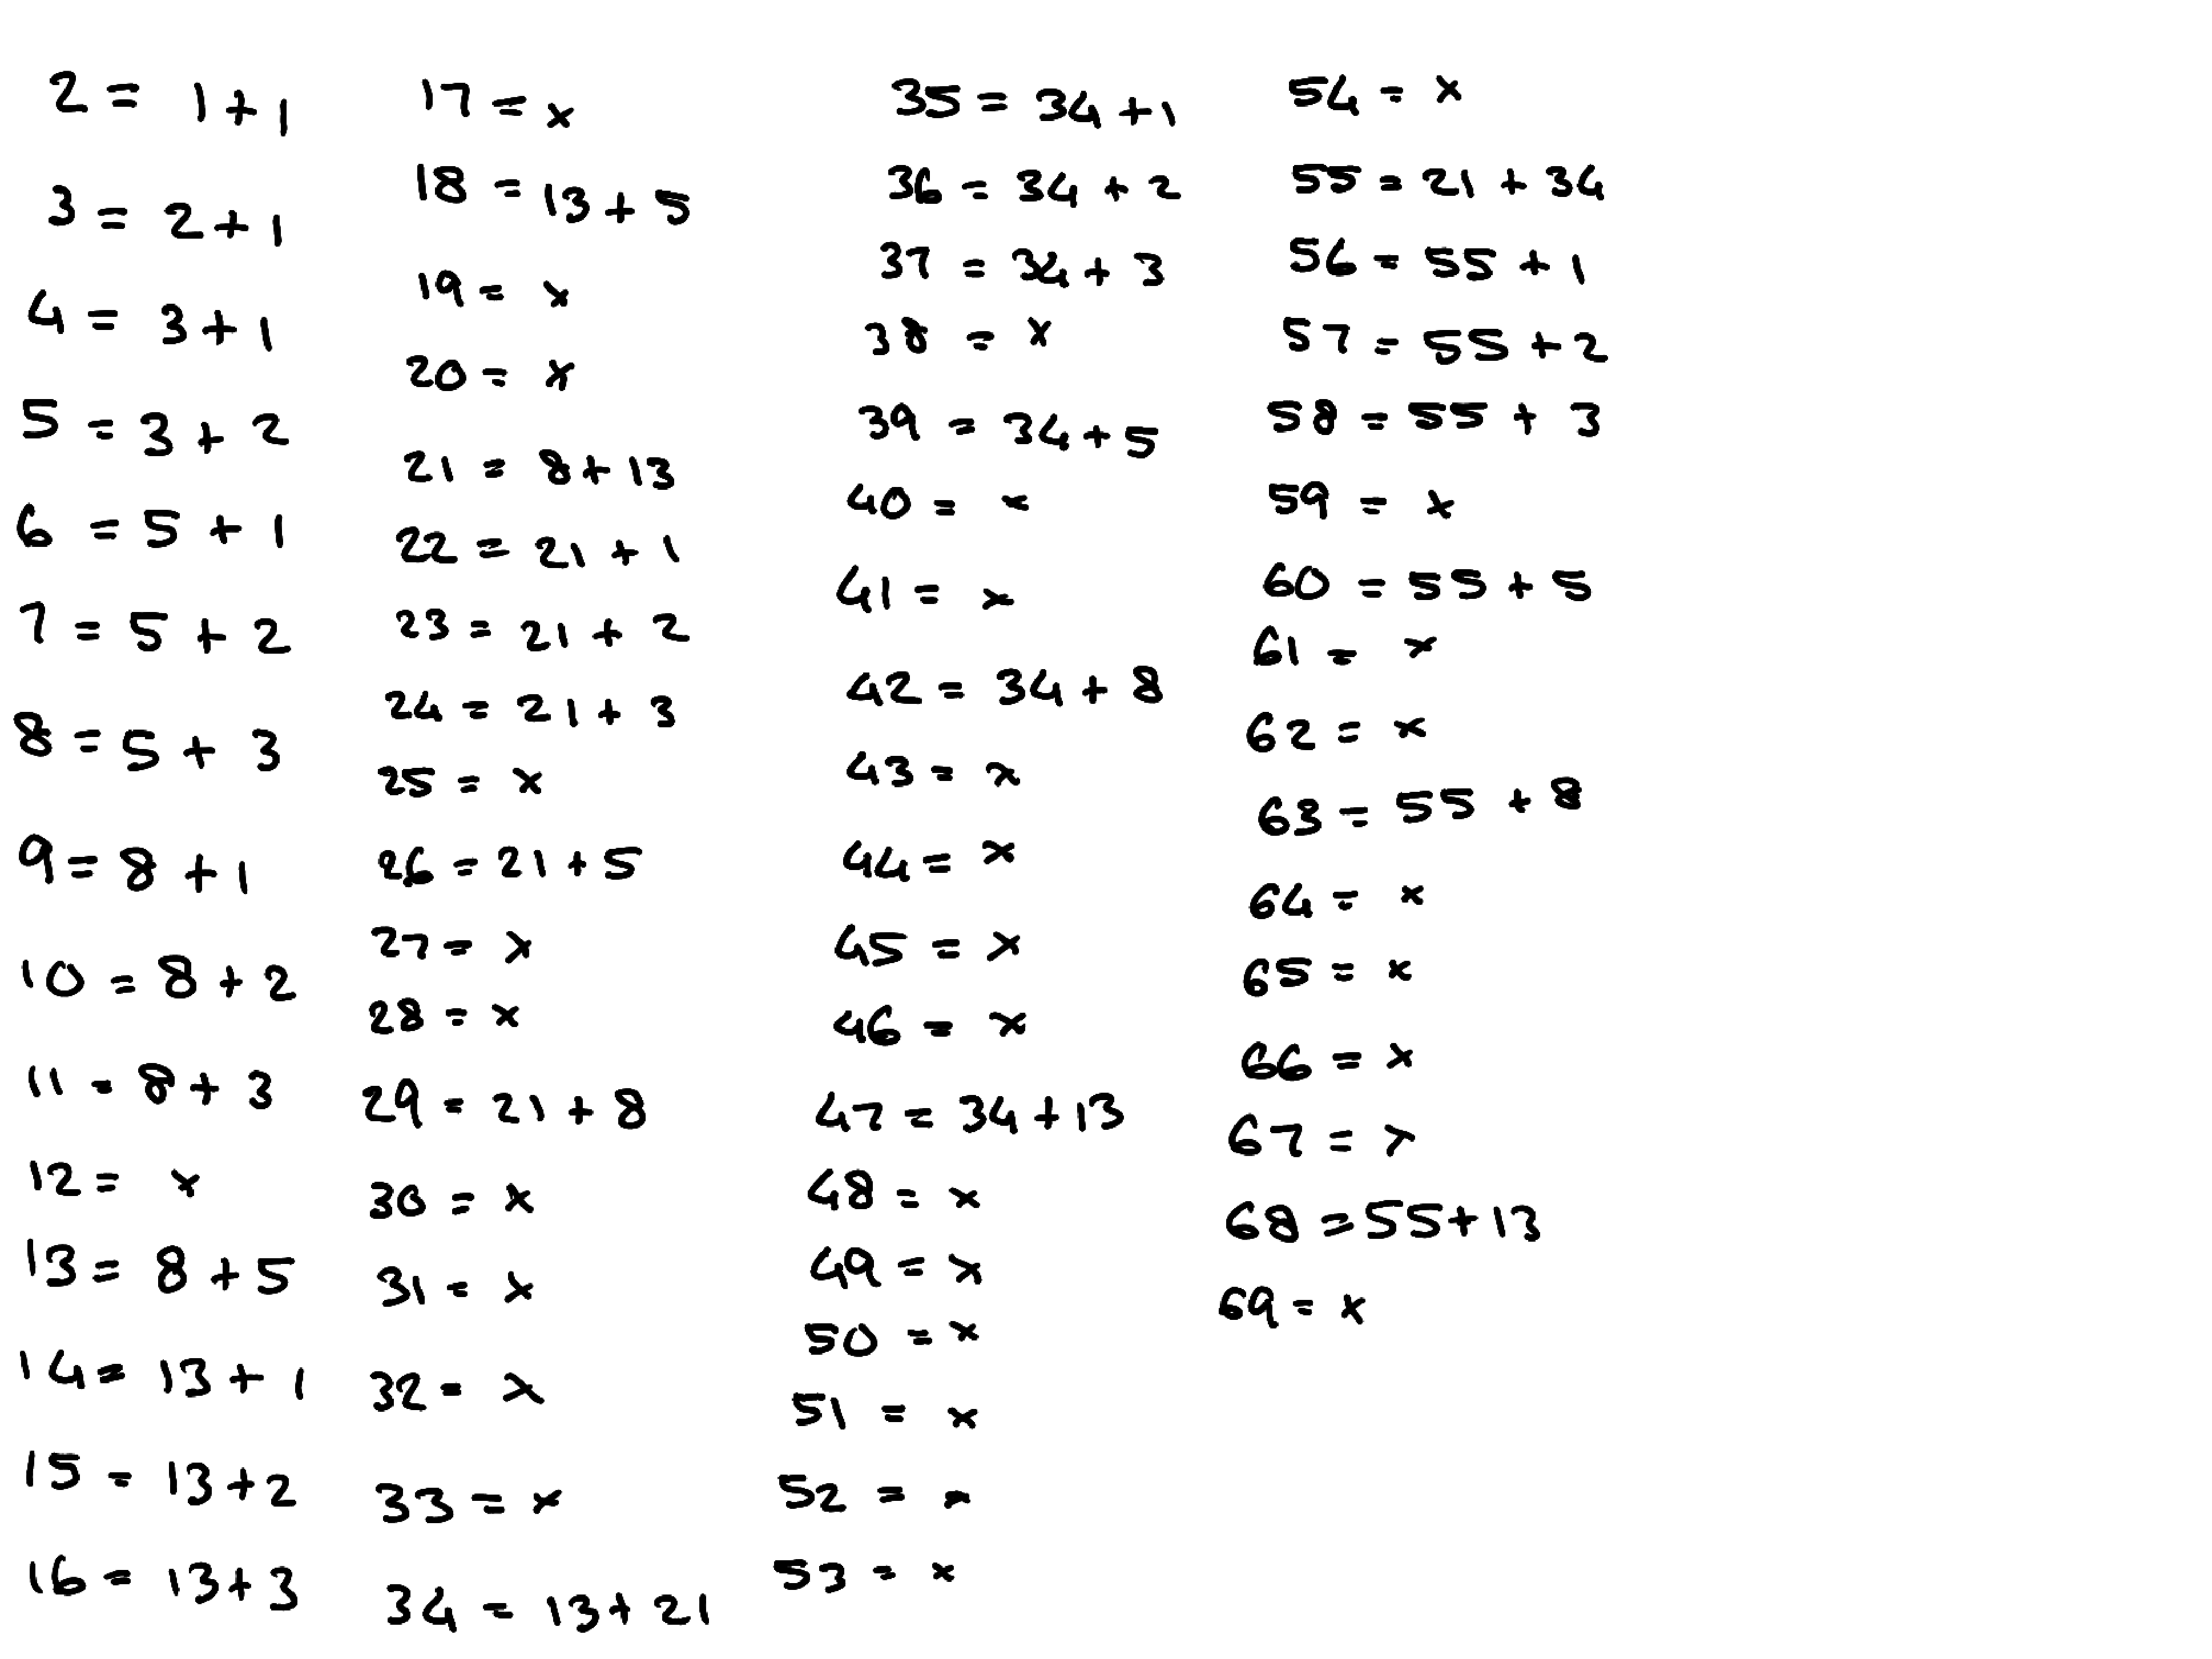
\includegraphics[width=0.7\textwidth]{Working.pdf}
\par
}

I noticed the following. If we order the elements of $F + F$ then
it "usually" looks like
$$
F_n, \ F_n + F_1, \ F_n + F_2, \ \ldots, \ F_n + F_{n-1}.
$$
I also see that, apart from some small values, most numbers cannot be
expressed as the sum of two fibonacci numbers. \vspace{0.2cm}

From this point on I changed my mindset about this problem. There is a
large class of mathematics problems that can be solved by the technique of
"spot this pattern and win", but looking at the data of this problem, it
seems that there are no real patterns. The number 6 in the problem
statement seems rather arbitrary, and it could very well be that case
that the set of fibonacci numbers is a red herring. It leads me to think
that the following statement might be true,
\vspace{0.2cm}

Let $S$ be an infinite set of positive integers. Let $S'$ be a set such that
if $a,b \in S$ (not necessarily distinct), then $a + b \in S'$.
Then there are infinitely many arithmetic progressions of length $k$ in
$S'$.
\vspace{0.2cm}

In particular for our problem we want to show the statement for $k = 6$.
This is a hard problem. Let's instead try and prove/disprove the smallest
case, that is $k = 3$. In fact when $k = 3$ the problem becomes easy
(relatively speaking). Here are the details.
\vspace{0.2cm}

Suppose the numbers $a$ and $a + \delta$ are both in $S$. Also the numbers
$$
(a) + (a) = 2a, \quad (a) + (a + \delta) = 2a + \delta, \quad
(a + \delta) + (a + \delta) = 2a + 2\delta
$$
are all in $S'$. This is an arithmetic progression of length 3, done!
\vspace{0.2cm}

Now what about $k = 4$? I'm pretty sure that the statement is false for
$k \geq 4$ after some expirementation. Back to the drawing board then.
\vspace{0.2cm}

I remember from Noether Sheet 6, the following identity
$3F_n = F_{n+2} + F_{n-2}$. So both $2F_n,\ 3F_n \in F+F$. It is natural
to hope that maybe $4F_n, 5F_n$ etc appear in $F+F$, but again after some
experimentation I don't believe these multiples of $F_n$ occur "regularly".
After a while of messing around I came across the fact that
$$
F_{n-3}, \ F_{n-1}, \ F_n, \ F_n + F_{n-2}
$$
are all in $F+F$ for large enough $n$ and this sequence is an AP with
common difference $F_{n-2}$. If we can show that it's possible to get
"lucky" infinitely often, that is find solutions to
$$
F_n + 2F_{n-2} = \text{Sum of two fibonacci numbers}
$$
$$
F_n + 3F_{n-2} = \text{Sum of two fibonacci numbers}
$$
then we would be done.
For the first equation I naturally considered the following table

{
\centering
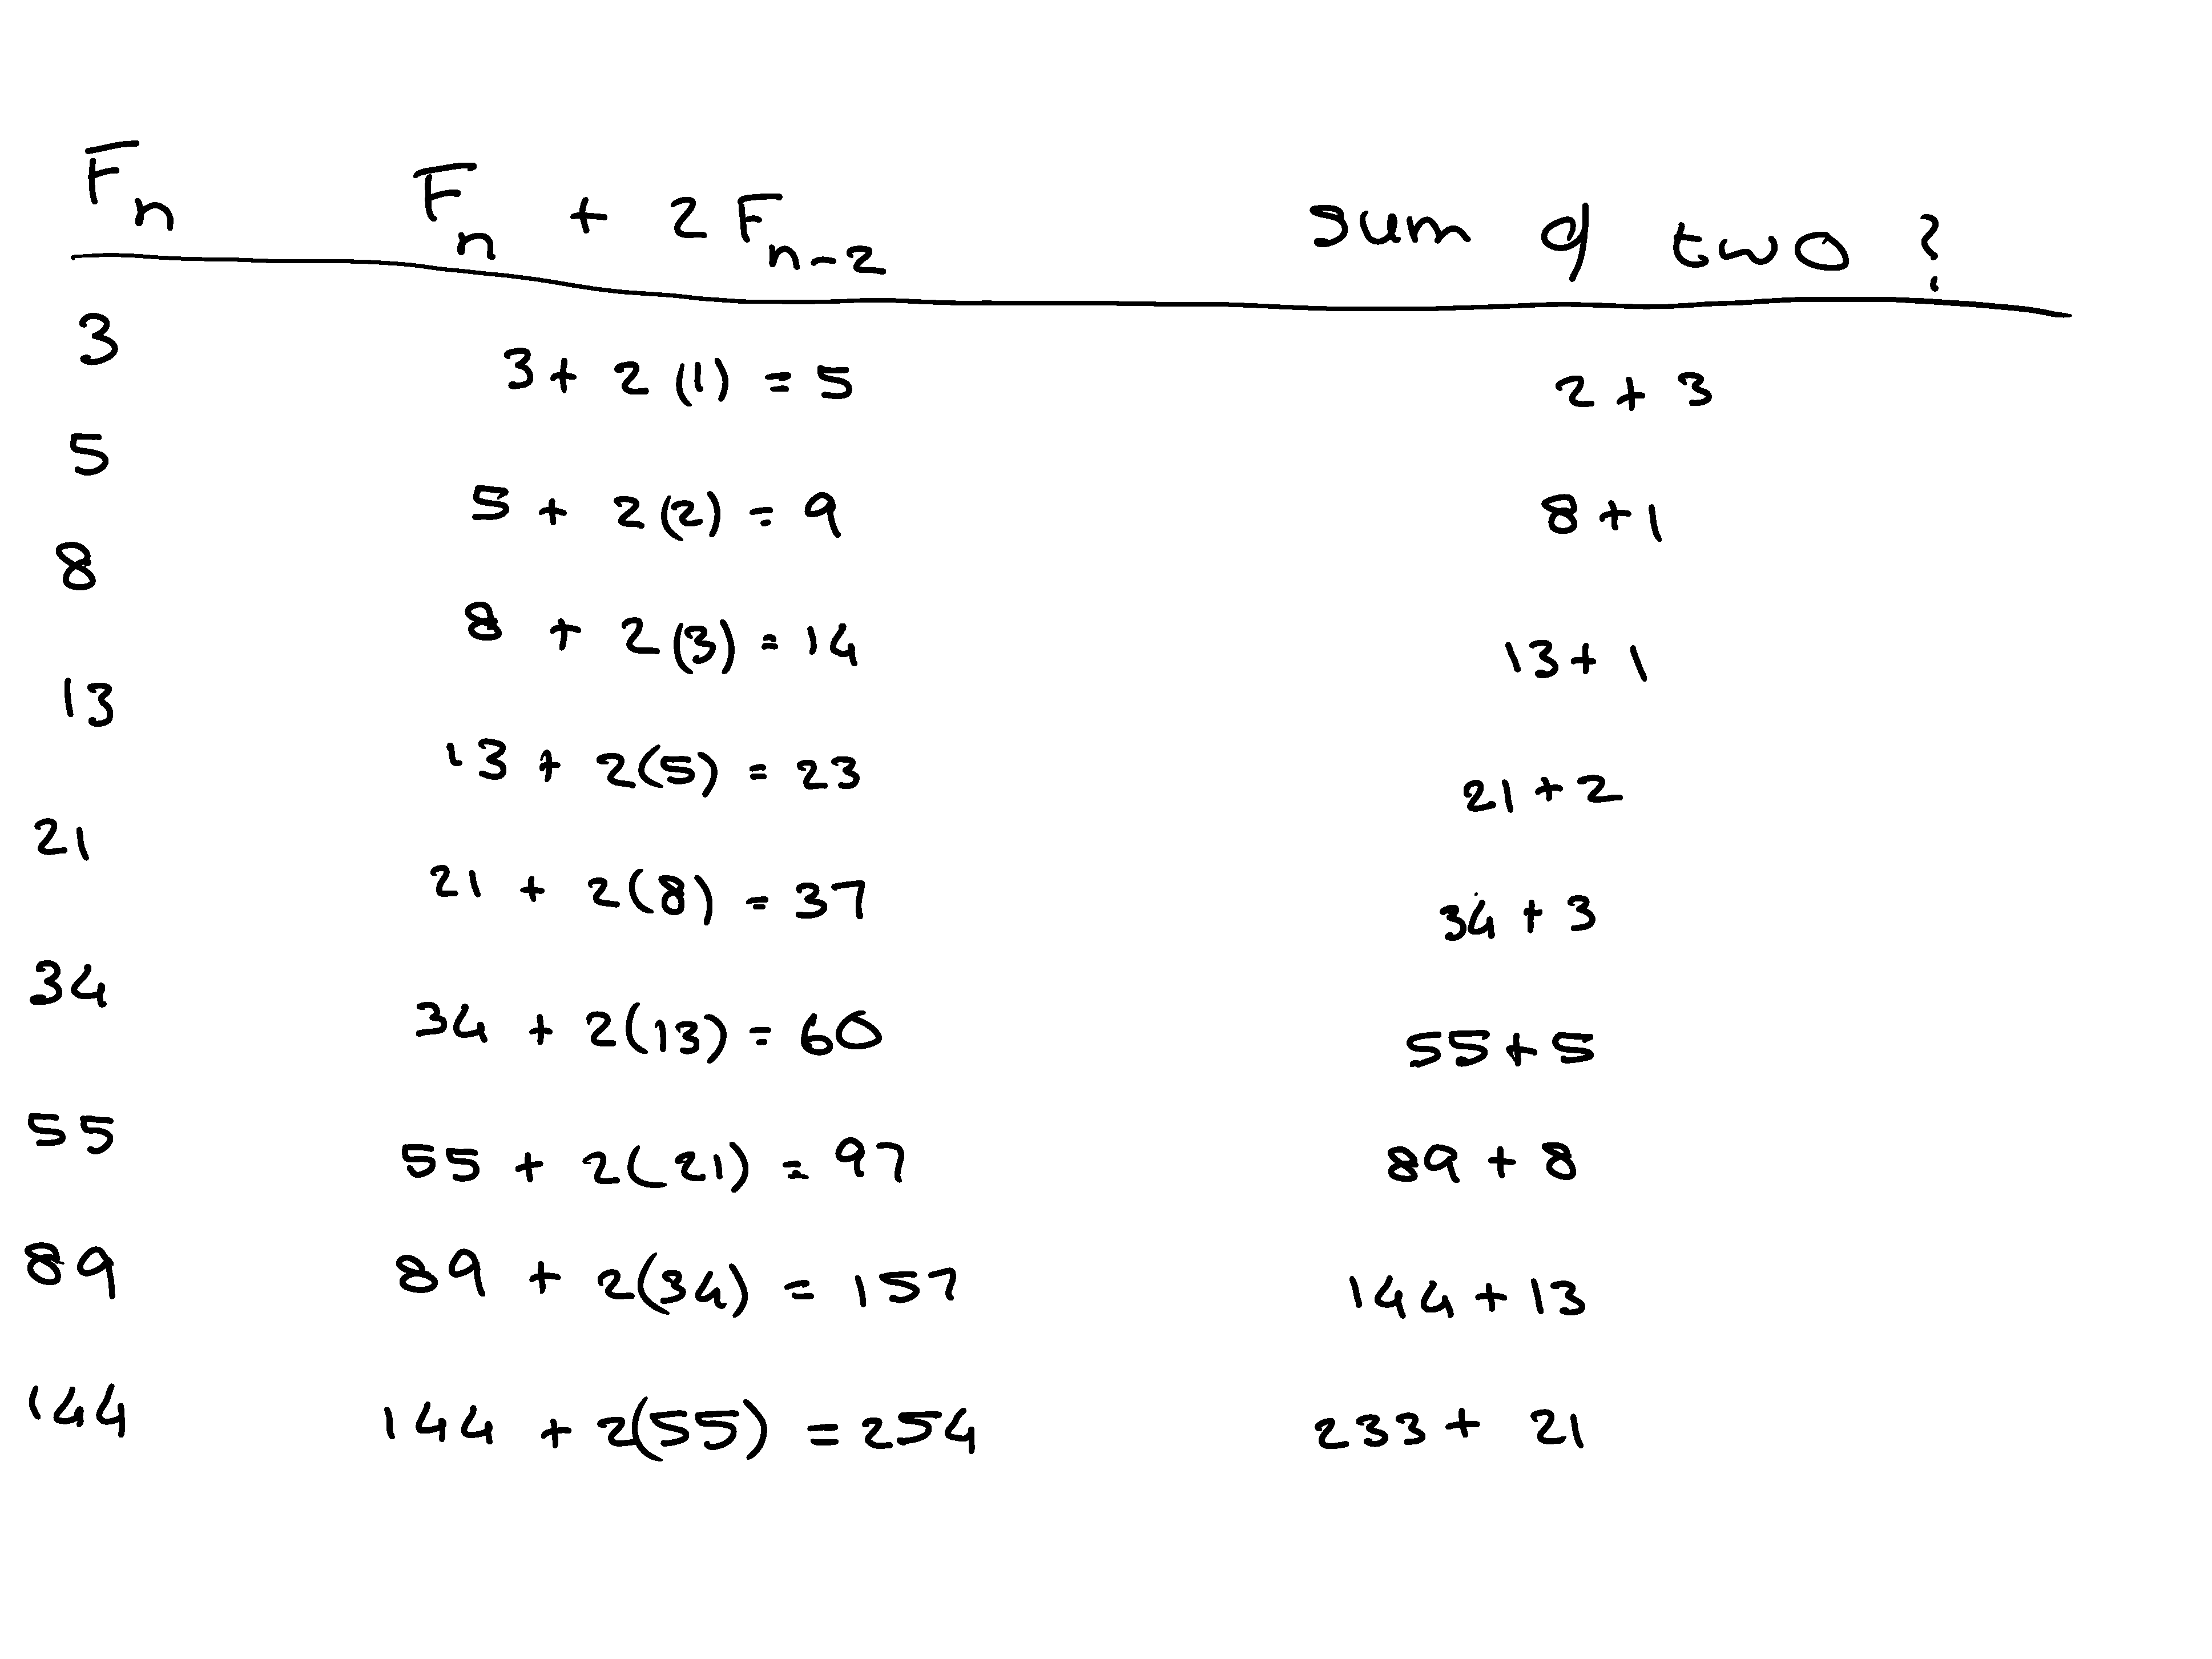
\includegraphics[width=0.7\textwidth]{Table.pdf}
\par
}

I continued this until $F_n = 1597$ and every time it was possible to
express $X = F_n + 2F_{n-2}$ as the sum of two fibonacci numbers, so it's
very likely that there is an identity to always express $X$ as the sum of
two fibonacci numbers. After looking at the table we conjecture that
$F_n + 2F_{n-2} = F_{n+1} + F_{n-4}$, and it's quite easy to show that
this result is true. The last part is just to express
$F_n + 3F_{n-2}$ as the sum of two fibonacci numbers. Unfortunately
if we try to make the same table for $F_n + 3F_{n-2}$ it seems that
usually numbers of this form can't be expressed as the sum of two fibonacci
numbers.\\

Finally after the hint to look at the $a + \delta$ logic but just replace
this with fibonacci numbers and their identities I found a working
construction. That is
$$
\underbrace{F_{n-4}}_{= 2F_{n-2} - F_{n-1}}, \
F_{n-2} + F_{n-2}, \
F_n + F_{n-2}, \
F_n + F_n, \
F_n + F_{n+1}, \
F_{n+1} + F_{n+1}
$$
which is an AP of length 6, with common difference $F_{n-1}$.
\end{hint}

\newpage

\begin{solution}{Solution}
We show the desired result by a construction. \vspace{0.2cm}

\textit{Claim 1: Let $n \geq 4$ be an integer. Then
$F_{n-4} = 2F_{n-2} - F_{n-1}$.} \vspace{0.2cm}

\textit{Proof:} Observe that the RHS is
\[
\begin{aligned}
2F_{n-2} - F_{n-1} &= F_{n-2} + (F_{n-2} - F_{n-1}) \\
&= F_{n-2} + (F_{n-2} - [F_{n-2} + F_{n-3}]) \\
&= F_{n-2} - F_{n-3} \\
&= F_{n-4}
\end{aligned}
\]
as desired. $\square$
\\

Let $n \geq 6$ be an integer. Then notice that we can write
$F_{n-4} = F_{n-5} + F_{n-6}$.
Now consider the following sequence.
$$
F_{n-5} + F_{n-6}, \quad F_{n-2} + F_{n-2}, \quad F_n + F_{n-2}, \quad
F_n + F_n, \quad F_n + F_{n+1}, \quad F_{n+1} + F_{n+1}.
$$
Each term is $F_{n-1}$ more than the last and clearly all 6 terms are in
$F+F$. Thus there are infinitely many AP's of length 6 in $F+F$.
$\blacksquare$ \\

\textit{Comments: Although the solution is really short this really isn't
an easy problem.}
\end{solution}
\newpage

\begin{problem}{Problem 5}
In triangle $ABC$, the angle $\angle BAC$ is trisected by $AD$ and $AE$,
where $D$ and $E$ lie on $BC$. Suppose that $BD = 2$, $DE = 3$ and
$EC = 6$. \vspace{0.2cm}

What is the length of $AC$?
\end{problem}

\begin{solution}{Solution}
We have the diagram

\begin{center}
\begin{asy}
/* Geogebra to Asymptote conversion, documentation at artofproblemsolving.com/Wiki go to User:Azjps/geogebra */
import graph; size(180);
real labelscalefactor = 0.5; /* changes label-to-point distance */
pen dps = linewidth(0.7) + fontsize(10); defaultpen(dps); /* default pen style */
pen dotstyle = black; /* point style */
real xmin = -2.870811382833745, xmax = 11.837832323636132, ymin = -1.1362011893428834, ymax = 12.439173471793133;  /* image dimensions */

pair A = (0.,0.), B = (6.324555320336759,0.), C = (10.672687103068286,10.104145188980606), D = (7.1151247353788545,1.837117307087383);
/* draw figures */
draw(A--C);
draw(B--A);
draw(A--D,  linetype("4 4"));
draw(A--(8.300978857941999,4.5927932677184575),  linetype("4 4"));
draw(B--D);
draw(D--(8.300978857941999,4.5927932677184575));
draw((8.300978857941999,4.5927932677184575)--C);
/* dots and labels */
dot(A,linewidth(4.pt) + dotstyle);
label("$A$", (-7.21818300648049e-4,0.11621523425367525), NW * labelscalefactor);
dot(B,dotstyle);
label("$B$", (6.391270735149042,0.14665329403200714), NE * labelscalefactor);
dot(C,linewidth(4.pt) + dotstyle);
label("$C$", (10.728694253561331,10.221651080659857), NE * labelscalefactor);
label("$2y$", (5.4933479716882525,4.879771589562614), NE * labelscalefactor);
label("$x$", (3.149617368756699,-0.1531865032561687), NE * labelscalefactor);
dot(D,linewidth(4.pt) + dotstyle);
label("$D$", (7.18266028938567,1.9577178508427537), NE * labelscalefactor);
dot((8.300978857941999,4.5927932677184575),linewidth(4.pt) + dotstyle);
label("$E$", (8.354525590851447,4.712362260781788), NE * labelscalefactor);
label("$y$", (3.606188265431677,0.6945383700419808), NE * labelscalefactor);
label("$\frac{3}{2}x$", (4.260606550665812,2.0946891198452473), NE * labelscalefactor);
label("$2$", (6.939155811159015,0.8315096390444743), NE * labelscalefactor);
label("$3$", (7.9283927539548005,3.129583152308531), NE * labelscalefactor);
label("$6$", (9.709019250987215,7.2539402522725), NE * labelscalefactor);
clip((xmin,ymin)--(xmin,ymax)--(xmax,ymax)--(xmax,ymin)--cycle);
/* end of picture */
\end{asy}
\end{center}

Denote $x = AB$ and $y = AD$. We are going to justify the other lengths
with this theorem.
\vspace{0.2cm}

\textit{Angle Bisector Theorem: Let $\triangle ABC$ have a bisector
$AD$, where $D$ lies on $BC$. Then $DB : DC = AB : AC$.} \vspace{0.2cm}

\textit{Proof:} Consider,

\begin{center}
\begin{asy}
/* Geogebra to Asymptote conversion, documentation at artofproblemsolving.com/Wiki go to User:Azjps/geogebra */
import graph; size(140);
real labelscalefactor = 0.5; /* changes label-to-point distance */
pen dps = linewidth(0.7) + fontsize(10); defaultpen(dps); /* default pen style */
pen dotstyle = black; /* point style */
real xmin = -1.18824549337867, xmax = 8.239101219059293, ymin = -1.5253289666699543, ymax = 9.437271238306808;  /* image dimensions */
pen ttttff = rgb(0.2,0.2,1.); pen qqzzqq = rgb(0.,0.6,0.);
pair A = (0.,0.), B = (7.,0.), C = (5.,8.), D = (6.148106603780189,3.407573584879245);

filldraw(arc(A,0.6261255697298993,360.,388.99730839595827)--(0.,0.)--cycle, ttttff + opacity(0.25),  ttttff);
filldraw(arc(A,0.6261255697298993,388.99730839595827,417.99461679191654)--(0.,0.)--cycle, ttttff + opacity(0.25),  ttttff);
filldraw(arc(D,0.6261255697298993,-151.00269160404176,-75.96375653207353)--(6.148106603780189,3.407573584879245)--cycle, qqzzqq + opacity(0.10000000149011612),  qqzzqq);
filldraw(arc(D,0.6261255697298993,104.03624346792648,208.99730839595827)--(6.148106603780189,3.407573584879245)--cycle, qqzzqq + opacity(0.10000000149011612),  qqzzqq);
/* draw figures */
draw(A--B);
draw(C--B);
draw(C--A);
draw(A--D);
/* dots and labels */
dot(A,dotstyle);
label("$A$", (0.05735706467707557,0.15315875549320632), NE * labelscalefactor);
dot(B,dotstyle);
label("$B$", (7.069963445651947,0.15315875549320632), NE * labelscalefactor);
dot(C,dotstyle);
label("$C$", (5.066361622516269,8.151912908792674), NE * labelscalefactor);
dot(D,linewidth(4.pt) + dotstyle);
label("$D$", (6.209040787273335,3.5342368320346647), NE * labelscalefactor);
label("$\alpha$", (0.6991357736502223,0.1375056162499588), NE * labelscalefactor,ttttff);
label("$\alpha$", (0.5112981027312525,0.4818746796014036), NE * labelscalefactor,ttttff);
label("$\beta$", (5.742937420138128,2.5020300977642496), NE * labelscalefactor,qqzzqq);
label("$180-\beta$", (4.307239875705497,3.5029305535481696), NE * labelscalefactor,qqzzqq);
clip((xmin,ymin)--(xmin,ymax)--(xmax,ymax)--(xmax,ymin)--cycle);
/* end of picture */
\end{asy}
\end{center}

By sine rule
$$
\frac{DB}{\sin \alpha} = \frac{AB}{\sin \beta}, \quad \quad
\frac{CD}{\sin \alpha} = \frac{AC}{\sin (180 - \beta)} = \frac{AC}{\sin \beta}
$$
We can re-arrange to get
$$
\frac{DB}{AB} = \frac{CD}{AC} = \frac{\sin \alpha}{\sin \beta} \
\Rightarrow \
\frac{DB}{DC} = \frac{AB}{AC}. \ \blacksquare
$$
\\

Now since $AD$ bisects $\angle BAE$ we deduce that $AE = \frac32 x$.
Similarly we find that $AC = 2y$.
\vspace{0.2cm}

Now by applying Cosine rule on $\triangle ADB, \triangle ADE$ and
$\triangle AEC$ we have the following equations
\[
\begin{aligned}
4 &= x^2 + y^2 - 2xy \cos \theta \\
9 &= \frac94 x^2 + y^2 - 3xy \cos \theta \\
36 &= \frac94 x^2 + 4y^2 - 6xy \cos \theta
\end{aligned}
\]
Now one can use whatever method they like to solve this system
in terms of $x^2, y^2$ and $xy\cos \theta$, I'll use matrices.
$$
\begin{bmatrix}
1 & 1 & -2 \\
9/4 & 1 & -3 \\
9/4 & 4 & -6
\end{bmatrix}
\begin{bmatrix}
x^2 \\ y^2 \\ xy\cos \theta
\end{bmatrix}
=
\begin{bmatrix}
4 \\ 9 \\ 36
\end{bmatrix}
$$

$$
\begin{bmatrix}
x^2 \\ y^2 \\ xy\cos \theta
\end{bmatrix}
=
\begin{bmatrix}
40 \\ 54 \\ 45
\end{bmatrix}
$$
which yields $x = 2\sqrt{10}, y = 3\sqrt6$ and $\cos \theta = \sqrt{15}/4$.
Finally the problem asked us for the length of $AC$ which is
$2y = 6\sqrt6$. $\blacksquare$
\end{solution}
\newpage

\begin{problem}{Problem 6}
If $x, y$ and $z$ are non-negative numbers, prove that at least one of
$x - xy$, $y - yz$ and $z - zx$ is at most $\frac14$.
\end{problem}

\begin{solution}{Solution}
Assume the contrary, that is
$$
x(1-y) > \frac14, \quad y(1-z) > \frac14, \quad z(1-x) > \frac14
$$
Then multiply all three ineqaulties together to get
$$
x(1-x)y(1-y)z(1-z) > \frac{1}{64}.
$$
Define $f(x) = x(1-x)$. It is routine to check that $f$ has a maxima
when $x=\frac12$ yielding $f(1/2) = 1/4$. So we deduce that
$$
\frac{1}{64} < x(1-x)y(1-y)z(1-z) \leq \frac{1}{64}.
$$
but this implies that
$$
\frac{1}{64} < \frac{1}{64}
$$
a contradiction! $\blacksquare$
\end{solution}
\newpage

\begin{problem}{Problem 7}
An unreliable postman has seven letters to deliver, one to each of seven
houses. In how many ways can they do this such that no house receives the
correct letter?
\end{problem}

\begin{solution}{Solution}
First we remove all creative sparkle from the problem. Let $f(n)$
count the number of permutations $\sigma$ of $\{1,2,\ldots, n\}$ such
that $\sigma$ has no fixed points. The problem is just asking us to compute
$f(7)$. \vspace{0.2cm}
Let $c(n)$ count the number of permutations $\sigma$ of
$\{1,2,\ldots, n\}$ such that $\sigma$ has no cycles of length $<n$
and no fixed points. It will prove useful to us to find a closed form
for $c(n)$.
\vspace{0.2cm}

\textit{Claim 1:} $c(n) = (n-1)!$. \vspace{0.2cm}

\textit{Proof:} Call a permutation $\sigma$ of $\{1,2,\ldots, n\}$
\textit{nice} if it has no cycles of length $< n$ and no fixed points.
Suppose that the permutation $\sigma$ is nice,
notice that the following is true. For any $x \in \{1,2,\ldots, n\}$,
the smallest integer $k$ satisfying $\sigma^k (x) = x$ is $k = n$.
This is because if $k < n$ then we have found a cycle of length $< n$.
This implies that
$$
\{ \sigma(1), \ \sigma^2(1), \ \ldots, \ \sigma^n(1) \}
=
\{ 1,2,\ldots, n \} \quad (*)
$$
and also the same is true when all the $\sigma^k (1)$'s are replaced with
$\sigma^k (x)$ for any $x = 1,2,\ldots,n$.
We know that $\sigma^n (1)$ must be $=1$, but otherwise we can choose the
values of $\sigma(1), \sigma^2(1), \ldots, \sigma^{n-1}(1)$ freely, they
just have to form a permutation of $\{2,3,\ldots,n\}$.
There are $(n-1)!$ ways to do so, to finish we should show that this action
also uniquely determines the values of
$\sigma(2), \sigma(3), \ldots, \sigma(n)$.
\vspace{0.2cm}

For any $x = 2,3,\ldots,n$ there exists a unique $k = 1,2,\ldots,(n-1)$
such that $\sigma^k (1) = x$ due to $(*)$. Thus
$\sigma(x) = \sigma^{k+1}(1)$ and since
$\sigma^2(1), \sigma^3(1), \ldots, \sigma^n(1)$ are all distinct
(again due to $(*)$) we have indeed uniquely determined
$\sigma(2), \sigma(3), \ldots, \sigma(n)$. $\square$ \\

Let $\sigma$ be a permutation of $\{1,2,\ldots, 7\}$ such that
$\sigma$ has no fixed points. Since it has no fixed points any cycles
in $\sigma$ must have length $ > 1$. It can be checked that there are
exactly four ways to organise the number of cycles in $\sigma$, they are
$$
(7), \ (2,2,3), \ (2,5), \ (3,4).
$$
So that means we could have one cycle of length 7, or two cycles of length
2 with one cycle of length 3, etc... From here we have all we need to
compute $f(7)$,
\[
\begin{aligned}
f(7) &= \binom{7}{7}\cdot c(7) + \binom{7}{2} \binom{5}{2} \binom{3}{3}
\cdot c(2) \cdot c(2) \cdot c(3) \\ &+
\binom{7}{2}\binom{5}{5} \cdot c(2) \cdot c(5) +
\binom{7}{3}\binom{4}{4} \cdot c(3) \cdot c(4) \\
&= 2064. \ \blacksquare
\end{aligned}
\]
\\

{\color{gray} \hline}
\vspace{0.2cm}

\textit{Addendums (after having read solutions).}\\

After seeing that my solution was wrong I tried the problem again.
Call a permutation \textit{nice} if it has no fixed points. \\

\textit{Claim 1:} Consider the permutations $\sigma_1, \sigma_2, \ldots,
\sigma_{n!}$ of $\{1,2,\ldots,n\}$. The $(n+1)!$ permutations of
$\{1,2,\ldots, n+1\}$ can be generated via the following algorithm.

\begin{enumerate}
\item For each permutation $\sigma_i$, ($i=1,2,\ldots, n!$) do the
following,
\item For each $(k=1,2,\ldots, (n+1))$ create a new permutation,
call it $\mu_{i,k}$ such that $\mu_{i,k}(n+1) = k$ and
$\mu_{i,k}(k) = n+1$ and for all other
$(x=1,2,\ldots,(n+1)), x \neq (n+1), x\neq k$
set $\mu_{i,k}(x) = \sigma_{i}(x)$. \vspace{0.2cm}

Informally that is to let $\mu_{i,k}$ swap
the position of $k$ and $(n+1)$ and for all the other numbers $x$ let
$\mu_{i,k}(x) = \sigma_i(x)$.
\end{enumerate}

\textit{Proof:} The algorithm loops over $n! \times (n+1)$ times and so
creates $(n+1)!$ permutations of length $(n+1)$. Consider the permutations
generated $\mu_{1,1}, \mu_{1,2}, \ldots, \mu_{n!, (n+1)}$. We must show that
the permutations in this list are pairwise distinct.
Define
$S_i = \{ \sigma_i(t) : t=1,2,\ldots,n \}$ and
$S_j = \{ \sigma_j(t) : t=1,2,\ldots,n \}$. \vspace{0.2cm}

First we show that if $i \neq j$ then $\mu_{i,x} \neq \mu_{j,y}$.
Note that $\sigma_i$ and $\sigma_j$ are not the same permutation.
There must exist (at least) two different numbers $1\leq a,b\leq n$ such that
$$
\sigma_i(a) \neq \sigma_j(a) \ \text{ and } \ \sigma_i(b) \neq \sigma_j(b).
$$
To see why note that if
there was only one number $k$ such that $\sigma_i(k) \neq \sigma_j(k)$,
then $| S_i \cap S_j | = n-1$.
Since permutations are surjective, both $|S_i| = n$ and $ |S_j| = n$. Then
it is a well-known fact that
\[
\begin{aligned}
|S_i \cup S_j| &= |S_i| + |S_j| - |S_i \cap S_j| \\
&= n + n - (n-1)\\
&= n+1
\end{aligned}
\]
but $|S_i \cup S_j|$ should be $=n$, contradiction. Now back to the main
goal, since $a \neq b$ at least one of $a,b$ is not equal to $k$. Suppose
WLOG that $a \neq k$. Then because of how the algorithm constructs
permutations we have that $\mu_{i,x}(a) \neq \mu_{j,y}(a)$. This is because
both $\mu_{i,x}(a)$ and $\mu_{j,y}(a)$ will be defined to be
$\sigma_i(a),  \sigma_j(a)$ respectively, as can be seen in the latter part
of step 2 of the algorithm.\vspace{0.2cm}

Next we show that if $x\neq y$ then $\mu_{i,x} \neq \mu_{j,y}$. This
proof is much easier than the last case, just note that
$\mu_{i,x}(x) = n+1$ whilst $\mu_{j,y}(y) = n+1$ and since $x\neq y$ they
clearly aren't the same permutation. \vspace{0.2cm}

So we have shown that if $\mu_{i,x} = \mu_{j,y}$ then $i = j$ and $x = y$.
This guarentees that the $(n+1)!$ permutations generated are in fact
pairwise distinct, as desired.
$\square$ \\

Consider some step of the algorithm when the permutation $\sigma_i$ has
$> 1$ fixed point. We claim that no nice permutations $\mu_{i,k}$
can be generated for this $i$. Suppose that $a,b$ are fixed points of
$\sigma_i$ permutation. Formally $\sigma_i(a) = a$ and $\sigma_i(b) = b$.

\begin{itemize}
\item If $k$ is not equal to either of $a,b$ then
$\mu_{i,k}(a) = \sigma_i(a) = a$ and $\mu_{i,k}(b) = \sigma_i(b) = b$,
which is due to step 2 of the algorithm,
and so $\mu_{i,k}$ isn't nice.

\item If $k$ is equal to one of $a,b$, say WLOG $k = a$, then
$\mu_{i,k}(b) = \sigma(b) = b$, which is due to step 2 of the algorithm,
and so $\mu_{i,k}$ isn't nice.
\end{itemize}

Suppose $\sigma_i$ has exactly one fixed point $a$,
Informally we just need to ensure $\mu_{i,k}$ swaps the position of $a$ and
$(n+1)$ and then for all the remaining numbers setting
$\mu_{i,k}(x) = \sigma_i(x)$ guarentees no fixed points.
More formally, in order to get rid of
this fixed point in $\mu_{i,k}$ we need $k = a$ and that way we have
$\mu_{i,k}(a) = n+1$ and $\mu_{i,k}(n+1) = a$, and for the remaining numbers
$(x=1,2,\ldots,n), (x\neq k), (x\neq (n+1))$ we have
$\mu_{i,k}(x) = \sigma_i(x) \neq x$ since we assumed there
was only one fixed point in $\sigma_i$.  Thus we know that $\mu_{i,k}$ is
nice.
\vspace{0.2cm}

Suppose that $\sigma_i$ has no fixed points. Informally we are going
to note that if $\mu_{i,k}$ swaps $(n+1)$ with any other number then the
resulting permutation is still nice. More formally if we let
$k=1,2,\ldots,n$ the permutation $\mu_{i,k}$ is nice, because we will get
$\mu_{i,k}(k) = n+1$ and $\mu_{i,k}(n+1) = k$ and for the remaining numbers
$(x=1,2,\ldots,n), (x\neq k), (x\neq (n+1))$ we know that
$\mu_{i,k}(x) = \sigma_i(x) \neq x$ since $\sigma_i$ has no fixed points.
Thus $\mu_{i,k}$ is nice.\\

Hence if $f(n)$ is the number of nice permutations of length $n$ then,
\[
\begin{aligned}
f(n+1) &= \# \begin{pmatrix}
\text{Permutations of length } n \\
\text{with exactly 1 fixed point.}
\end{pmatrix}
+
\underbrace{
n \times \# \begin{pmatrix}
\text{Permutations of length } n \\
\text{with no fixed points.}
\end{pmatrix}
}_{\text{There are $n$ ways to pick the value of $\mu_{i,k}(n+1)$.}}
\end{aligned}
\]
For the first term notice that there are $n$ ways to choose where the
fixed point is in the permuation of length $n$ and then there are
$f(n-1)$ ways to permute the remaining $(n-1)$ numbers in such a way
that there are no fixed points. \vspace{0.2cm}

For the second term notice that the number of permutations of length $n$
with no fixed points is exactly $f(n)$. So we derive the recurrence
relation,
$$
f(n+1) = nf(n-1) + nf(n).
$$
We can compute by hand that $f(2) = 1, f(3) = 2$, then using our recurrence
\[
\begin{aligned}
f(4) &= 3(1) + 3(2) = 9 \\
f(5) &= 4(2) + 4(9) = 44 \\
f(6) &= 5(9) + 5(44) = 265 \\
f(7) &= 6(44) + 6(265) = 1854
\end{aligned}
\]
so our answer is 1854. $\blacksquare$
\end{solution}
\newpage

\begin{problem}{Problem 8}
In this question, we're going to prove \textit{Lagrange's four square
theorem,} which states that any positive integer can be written as the sum
of four squares. \vspace{0.2cm}

(a) Show that, if $x$ and $y$ are integers that can be written as the sum of
four squares, $xy$ can be written as the sum of four squares. \vspace{0.2cm}

(b) Suppose that $p$ is a prime number greater than 2. Show that there must
exist $a$ and $b$ with $0 \leq a,b \leq \frac{p-1}{2}$ such that
$a^2 + b^2 + 1 = np$ for some integer $n$. \vspace{0.2cm}

Explain why $1 \leq n < p$.
\vspace{0.2cm}

(c) Suppose that $m$ is the smallest positive integer such that $mp$ can
be written as the sum of four squares. Then, for $a_1, a_2, a_3$ and
$a_4$ integers, we can write
$$
mp = a_1^2 + a_2^2 + a_3^2 + a_4^2.
$$
Can you find integers $b_1, b_2, b_3$ and $b_4$ such that
$a_i \equiv b_i \ (\text{mod } m)$ and $b_1^2 + b_2^2 + b_3^2 + b_4^2 = mr$
with $0 \leq r \leq m$? \vspace{-0.2cm}

How can you write $m^2 pr$ as the sum of four squares? What about $pr$?
\vspace{0.2cm}

(d) Hence prove Lagrange's four square theorem.
\end{problem}

\begin{solution}{Solution}
(a) Let $x = a_1^2 + a_2^2 + a_3^2 + a_4^2$. Let
$y = b_1^2 + b_2^2 + b_3^2 + b_4^2$. Then
\[
\begin{aligned}
xy &= a_1^2 b_1^2 + a_1^2 b_2^2 + a_1^2 b_3^2 + a_1^2 b_4^2 \\
   &+ a_2^2 b_1^2 + a_2^2 b_2^2 + a_2^2 b_3^2 + a_2^2 b_4^2 \\
   &+ a_3^2 b_1^2 + a_3^2 b_2^2 + a_3^2 b_3^2 + a_3^2 b_4^2 \\
   &+ a_4^2 b_1^2 + a_4^2 b_2^2 + a_4^2 b_3^2 + a_4^2 b_4^2.
\end{aligned}
\]
Now it can be (painstakingly) checked that
\[
\begin{aligned}
xy &= (a_1 b_1 + a_2 b_2 + a_3 b_3 - a_4 b_4)^2 \\
&+ (a_1 b_3 + a_2 b_4 - a_3 b_1 + a_4 b_2)^2 \\
&+ (-a_1 b_2 + a_2 b_1 + a_3 b_4 + a_4 b_3)^2 \\
&+ (a_1 b_4 - a_2 b_3 + a_3 b_2 + a_4 b_1)^2
\end{aligned}
\]
and so $xy$ can be expressed as the sum of four squares. $\square$
\\

(b)
Since the problem talks about "some" integer $n$, it suffices to show that
there exist $a,b$ satisfying those inequalities and
$a^2 + b^2 \equiv -1 \ (\text{mod } p)$.
I am going to show that it suffices to solve the problem for
$0 \leq a,b \leq p-1$. Observe that modulo $p$ the following sets are the
same
$$
\{ 0,1,\ldots,p-1 \} = \left\{ 0, \pm1, \ldots, \pm\frac{p-1}{2} \right\}.
$$

Now let $0 \leq r \leq p-1$ be an integer. Due to our observation, modulo $p$
we can write $r \equiv k$ for some $0 \leq |k| \leq \frac{p-1}{2}$.
So $r^2 \equiv k^2 \equiv |k|^2 \ (\text{mod } p)$. Now if we pick
$0 \leq a \leq p-1$ we have shown by our previous arguement that there
must be some integer $0 \leq x \leq \frac{p-1}{2}$ such that
$a^2 \equiv x^2 \ (\text{mod } p)$, and we can say the same exact statement
again just replacing $a$ with $b$. Thus it is okay to just consider
$0 \leq a,b \leq p-1$. \vspace{0.2cm}

Now we are going to handle two cases, when $p \equiv 1 \ (\text{mod } 4)$
and when $p \equiv 3 \ (\text{mod } 4)$, since $p$ is an odd prime.
\\

{\color{gray} \hline}
\vspace{0.2cm}

\textit{Case 1:} $p \equiv 1 \ (\text{mod } 4)$. Then for some integer $k$
we may write $p = 4k + 1$. We are going to pick $a=0$ and then
show that $b^2 \equiv -1$ has a solution mod $p$. \vspace{0.2cm}

\textit{Claim 1: } $-1$ is a quadratic residue modulo $p$. \vspace{0.2cm}

\textit{Proof:} We are going to use the Legendre symbol and Euler's
criterion.
\[
\begin{aligned}
\left( \frac{p-1}{p} \right) &\equiv (p-1)^\frac{p-1}{2} \ (\text{mod } p)
\\
&\equiv (-1)^\frac{4k}{2} \equiv (-1)^{2k} \equiv 1 \ (\text{mod } p).
\end{aligned}
\]
Since the Legendre symbol evaluated to 1 mod $p$ and $-1 \equiv 1 \bmod p$
only when $p = 2$ and we have $p > 2$ we can conclude that
$\left(\frac{p-1}{p}\right) = 1$ and so, by definition of the Legendre
symbol, $p-1 \equiv -1$ is a quadratic
residue mod $p$. $\square$
\vspace{0.2cm}

Now set $a=0$. Now we just need to find $0 \leq b \leq p-1$ such that
$b^2 \equiv -1 \ (\text{mod } p)$, but such a $b$ is guarenteed to exist
due to claim 1. \\

{\color{gray} \hline}
\vspace{0.2cm}

\textit{Case 2:} $p \equiv 3 \ (\text{mod } 4)$. We may write $p = 4k + 3$
for some integer $k$. We are trying to find a pair of quadratic residues
of the form $(a^2, b^2) = (q,\ -1 - q)$ mod $p$, and we are going to show
that such a pair must exist via the Pigeonhole principle.
\vspace{0.2cm}

\textit{Claim 2: Amongst the non-zero residues mod $p$,
$\{1,2,\ldots,p-1\}$ there are exactly $\frac{p-1}{2}$ quadratic residues
mod $p$.}
\vspace{0.2cm}

\textit{Proof:} Let $1 \leq a \leq p-1$ be an integer. Using the
Legendre symbol and Euler's criterion we find
\[
\begin{aligned}
\left( \frac{a}{p} \right) \equiv a^\frac{p-1}{2} &\equiv a^{2k + 1} \
(\text{mod } p) \\
\left( \frac{p-a}{p} \right) \equiv (-a)^\frac{p-1}{2} &\equiv -a^{2k+1} \
(\text{mod } p)
\end{aligned}
\]
Now Euler's criterion guarentees that both expressions evaluate to one of
$\{-1,1\}$. Since the two expressions sum to 0 mod $p$ and $p > 2$ we can
conclude that exactly one of the two expressions evaluates to 1. Thus,
by definition of the Legendre symbol,
exactly one of $(a, -a)$ is a quadratic residue mod $p$. Now since the
non-zero residues mod $p$ can be expressed in the form
$\{ \pm k \ \mid \ k=1,2,\ldots,\frac{p-1}{2} \}$ we know that for each
$k$ precisely one of $(k, -k)$ is a square mod $p$, and thus there
are exactly $\frac{p-1}{2}$ quadratic residues amongst the non-zero residues
mod $p$. $\square$
\vspace{0.2cm}

Now since 0 is a quadratic residue, we can say that amongst
$\{0,1,\ldots,p-1\}$ there are exactly $\frac{p-1}{2} + 1 = \frac{p+1}{2}$
squares mod $p$ due to claim 2, and consequently
$\frac{p-1}{2}$ non-quadratic residues. Consider pairs of numbers
$(k, \ -1-k)$ where $k$ is a square mod $p$. Suppose FTSOC that
over all $\frac{p+1}{2}$ choices of $k$ the number $-1-k$ is a non-quadratic
residue. Note that $-1 - k_1 \equiv -1 - k_2 \iff k_1 \equiv k_2$ mod $p$,
so we have found $\frac{p+1}{2}$ pairwise distinct non-quadratic residues
mod $p$, but there should only be $\frac{p-1}{2}$, a contradiction.
Hence there has to exist a
pair of squares mod $p$ of the form $(a^2, b^2) = (q, \ -1-q)$.\\

{\color{gray} \hline}
\vspace{0.2cm}

Finally we explain the inequality on $n$.
Since $a, b \leq \frac{p-1}{2}$ we have
\[
\begin{aligned}
a^2 + b^2 + 1 &\leq \left( \frac{p-1}{2} \right)^2 +
                   \left( \frac{p-1}{2} \right)^2 +
                   1 \\
&= p^2 - 2p + 2 \\
np &\leq p^2 - 2p + 2 \\
n &\leq p - 2 + \frac{2}{p}
\end{aligned}
\]
and since $p \geq 3$ we have $n \leq p - \frac43 \Rightarrow n < p$.
Also since $a,b \geq 0$, we have $0^2 + 0^2 + 1 \leq np$ and so
$n \geq \frac{1}{p}$ but since $n \in \mathbb{Z}$ we have $n \geq 1$.
$\square$ \\

(c) Due to the division algorithm, we can write
$a_i = d_i m + r_i$ for $(i=1,2,3,4)$, where $d_i \in \mathbb{Z}$ and
integers $0 \leq r_i < m$. We have two cases.
\vspace{.2cm}


{\color{gray} \hline}
\vspace{0.2cm}

\textit{Case 1: $m$ is odd.} \vspace{0.2cm}

Then modulo $m$ the following is true,
$$
\{0,1,\ldots,m-1 \} = \left\{0,\pm 1, \ldots, \pm \frac{m-1}{2} \right\}.
$$
Thus for each $0 \leq r_i < m$ there is some integer $x_i$ satisfying
$0 \leq |x_i| \leq \frac{m-1}{2}$ and $r_i \equiv x_i \ (\text{mod } m)$.
Now for each $(i=1,2,3,4)$ define $b_i = x_i$. Then clearly
$a_i \equiv b_i \ (\text{mod } m)$ and
\[
\begin{aligned}
b_1^2 + b_2^2 + b_3^2 + b_4^2 &\leq \frac{(m-1)^2}{4} +
\frac{(m-1)^2}{4} + \frac{(m-1)^2}{4} + \frac{(m-1)^2}{4} \\
&= (m-1)^2 \\
&< m^2.
\end{aligned}
\]


{\color{gray} \hline}
\vspace{0.2cm}

\textit{Case 2: $m$ is even.} \vspace{0.2cm}

Then modulo $m$ the following is true,
$$
\{ 0,1,\ldots, m-1 \} = \left\{ 0, \pm 1, \ldots, \pm \frac{m}{2} \right\}.
$$
Thus for each $0 \leq r_i < m$ there is some integer $x_i$ satisfying
$0 \leq |x_i| \leq \frac{m}{2}$ and $r_i \equiv x_i \ (\text{mod } m)$.
Now for each $(i=1,2,3,4)$ define $b_i = x_i$. Clearly
$a_i \equiv b_i \ (\text{mod } m)$ and
\[
\begin{aligned}
b_1^2 + b_2^2 + b_3^2 + b_4^2 &\leq \frac{m^2}{4} +
\frac{m^2}{4} + \frac{m^2}{4} + \frac{m^2}{4} \\
&= m^2. \\
\end{aligned}
\]

{\color{gray} \hline}
\vspace{0.2cm}

Now since $a_i \equiv b_i \ (\text{mod } m)$ and
$a_1^2 + \cdots + a_4^2 \equiv 0 \ (\text{mod } m)$, we find that
$b_1^2 + \cdots + b_4^2$ is divisible by $m$.
Recall that from both cases we showed that
$b_1^2 + \cdots + b_4^2 \leq m^2$. Now for some integer $r$ we may write
$$
0 \leq b_1^2 + b_2^2 + b_3^2 + b_4^2 = mr \leq m^2
$$
which implies that $0 \leq r \leq m$, as desired. \\

Noting that $m^2pr = mp \times mr$, we can use the identity in (a) to write
\[
\begin{aligned}
m^2 pr &= (a_1 b_1 + a_2 b_2 + a_3 b_3 - a_4 b_4)^2 \\
&+ (a_1 b_3 + a_2 b_4 - a_3 b_1 + a_4 b_2)^2 \\
&+ (-a_1 b_2 + a_2 b_1 + a_3 b_4 + a_4 b_3)^2 \\
&+ (a_1 b_4 - a_2 b_3 + a_3 b_2 + a_4 b_1)^2.
\end{aligned}
\]
Now consider $mr = b_1^2 + \cdots + b_4^2$. Note that if we replace
$b_i \rightarrow -b_i$ the quantity $mr$ remains unchanged. So we can
choose the signs of the $b_i$'s as we wish. Let us replace $b_4$ with
$-b_4$ and now notice that
\[
\begin{aligned}
m^2 pr &= (a_1 b_1 + a_2 b_2 + a_3 b_3 + a_4 b_4)^2 \\
&+ (a_1 b_3 - a_2 b_4 - a_3 b_1 + a_4 b_2)^2 \\
&+ (-a_1 b_2 + a_2 b_1 - a_3 b_4 + a_4 b_3)^2 \\
&+ (-a_1 b_4 - a_2 b_3 + a_3 b_2 + a_4 b_1)^2.
\end{aligned}
\]
and then since $a_i \equiv b_i \ (\text{mod } m)$,
\[
\begin{aligned}
m^2 pr &\equiv (mp)^2
+ (0)^2
+ (0)^2
+ (0)^2 \ (\text{mod } m).
\end{aligned}
\]
and so every bracket is divisible by $m$. Thus for some integers
$c_1, c_2, c_3, c_4$ it is possible to write
\[
\begin{aligned}
m^2 pr &= m^2 c_1^2 + m^2 c_2^2 + m^2 c_3^2 + m^2 c_4^2 \\
pr &= c_1^2 + c_2^2 + c_3^2 + c_4^2
\end{aligned}
\]
and so we can also write $pr$ as the sum of four squares. $\square$
\\

(d) We begin with an important claim. Let the $a_i$'s and the $b_i$'s
be defined as they were in (c).\\

\textit{Claim 1: Let $p$ be a prime. It is possible to express $p$ as
the sum of four squares.} \vspace{0.2cm}

\textit{Proof:} Note that $2 = 1^2 + 1^2 + 0^2 + 0^2$, so from here on
assume that $p > 2$. Let $m$ be the smallest positive integer such that
$mp$ can be expressed as the sum of four squares. Let us suppose FTSOC that
$m > 1$. Owing to part (c) it is
also possible to find an integer $0 \leq r \leq m$ such that $pr$ can be
expressed as the sum of four squares.
\\

\textit{Case 1: $r = m$.} Again looking at part (c), this happens only when
$m$ is even and $a_i \equiv \pm \frac{m}{2} \equiv \frac{m}{2}
\ (\text{mod } m)$
(note that for even $m$ we have
$\pm \frac{m}{2} \equiv \frac{m}{2} \bmod m$) for every $(i=1,2,3,4)$. That
means there must be a sequence of integers $(k_i)_{i=1}^4$ such that
$a_i = k_i m + \frac{m}{2}$. Hence,
\[
\begin{aligned}
mp &= \left(k_1 m + \frac{m}{2}\right)^2 +
      \left(k_2 m + \frac{m}{2}\right)^2 +
      \left(k_3 m + \frac{m}{2}\right)^2 +
      \left(k_4 m + \frac{m}{2}\right)^2\\
&= m^2 (k_1^2 + k_2^2 + k_3^2 + k_4^2) + m^2 (k_1 + k_2 + k_3 + k_4) + m^2
\end{aligned}
\]
But this implies that $m^2 \mid mp \Rightarrow m \mid p$. Thus
$m \in \{1,p\}$. Since we assumed that $m > 1$, the only possibility is that
$m = p$. But now recall that part (b) guarenteed the existance of an
integer $1 \leq n < p$ satisfying $np = a^2 + b^2 + 1^2 + 0^2$ for some
$a,b\in \mathbb{Z}$, and so $m = p$ cannot be the smallest positive integer
such that $mp$ can be written as the sum of four squares, a contradiction.
\\

\textit{Case 2: $r=0$.} We have
$b_1^2 + \cdots + b_4^2 = 0$ If this happens then it must be the case that
$b_1 = b_2 = b_3 = b_4 = 0$, because if any one of the $b_i$'s
were $ > 0$ then the sum of their squares would be $ > 0$ also. Thus
$a_i \equiv b_i \equiv 0 \ (\text{mod } m)$. Hence, using the fact that
$m \mid a_i \Rightarrow m^2 \mid a_i^2$
$$
m^2 \mid (a_1^2 + a_2^2 + a_3^2 + a_4^2) = mp \ \Rightarrow \ m \mid p.
$$
Thus $m \in \{1,p\}$, and we can show that both cases yield a contradiction
using the same arguement found at the end of case 1.
\\

\textit{Case 3: $0 < r < m$.} Then in this case we have found a smaller
positive integer $r$ such that $pr$ can be expressed as the sum of four
squares, directly contradicting the definition of $m$ as the smallest
positive integer such that $mp$ can be written as the sum of four squares.
\\

In each case we found a contradiction, so it must be the case that $m=1$
or equivalently $p$ can be expressed as the sum of four squares. $\square$
\\

Now via the Fundamental theorem of arithmetic, we know that every positive
integer can be expressed as a product of some finite number of primes.
Then by repeatedly applying the lemma shown in part (a) of this problem
we can show that every positive integer can indeed be expressed as the
sum of four squares. $\blacksquare$
\end{solution}

\end{document}
